\documentclass[a4paper]{article}

\usepackage[pdftex]{graphicx}
\usepackage{a4wide}
\usepackage{hyperref}
\usepackage{times}

% TODO: get UTF to work in biblio (Normunds' citation)
%\usepackage[utf8]{inputenc}
%\usepackage[T1]{fontenc}

\graphicspath{{./images/}}

\def\uid#1{\texttt{#1}}
\def\xp#1{\texttt{#1}}
\newcommand\ace{Attempto Controlled English}

\begin{document}
\title{Attempto Controlled English in Grammatical Framework}
\author{DRAFT}

\hyphenation{alpha-numeric}
\hyphenation{ex-pe-ri-ment-al}

\maketitle
\begin{abstract}
This report describes the implementation of a large part of the
Attempto Controlled English (ACE) syntax ---
the subset of ACE that is accepted by AceWiki ---
in Grammatical Framework (GF) and making it available via [TODO: 10]
languages that are supported by the GF Resource Grammar Library (RGL).
The main goal of this work is to make ACE available in multiple languages
in order to allow
ACE-based knowledge representation also in languages other than English.
Additionally, having a GF implementation of the ACE language would provide
ACE users with new (GF-based) editing tools.
\end{abstract}

\section{Introduction}

\ace{} (ACE) \cite{fuchs:reasoningweb2008}
is a general purpose
first-order language (FOL)
with English syntax,
i.e. ACE can be viewed as both a natural language understandable by every
English speaker, as well as a formal language with a precisely defined
syntax and semantics understandable by automatic theorem proving software.
ACE texts are deterministically interpreted
via Discourse Representation Structures \cite{kamp:drt1993}.
The syntactically legal sentence structures and their
unambiguous interpretation is explained in the end-user documentation of
\emph{construction} and \emph{interpretation} rules.
The ACE toolchain includes a parser that maps ACE sentences into a concrete
DRS form \cite{ifi-2010.0010} and further into formats supported by existing
automatic reasoners (e.g. OWL, SWRL, TPTP).

End-users working with ACE can specify a lexicon that maps English
wordforms (nouns, verbs, adjectives, ...) into logical atoms, which the users
can interpret as they wish, but otherwise the ACE grammar or its mapping to
DRS cannot be changed.

Grammatical Framework (GF) \cite{ranta:book2011}
is a framework for defining multilingual grammars.

This paper is structured in the following way. In section ...

\section{Goals and requirements}

The overall goal of this work is to make ACE available to users who have little
English skills by turning ACE-based systems like
AceWiki \cite{kuhn2010doctoralthesis} multilingual. This allows users
to create and consume content whose native format is a formal language
(specifically a FOL-based language) in multiple natural languages
via an ACE-based interlingua (see figure \ref{fig:languages}).
Also, having a GF implementation of the ACE language would
provide ACE users with new (editing) tools that are based on the GF technology,
offering e.g. look-ahead editing, embeddable grammars, conversion into
speech recognition grammar formats, etc.

\begin{figure}[ht]
\centering
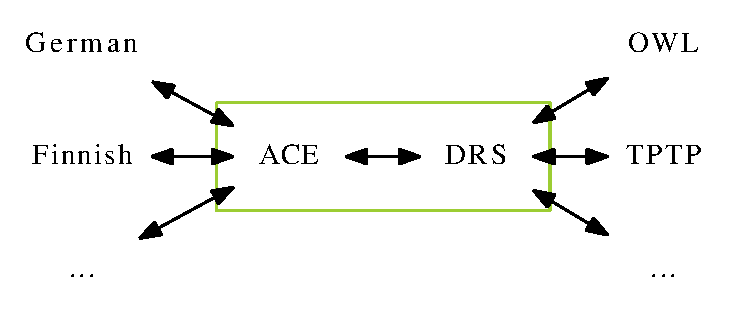
\includegraphics[width=0.7\textwidth]{languages}
\caption[Languages]
{Languages}
\label{fig:languages}
\end{figure}

Our main research questions are:

\begin{itemize}
\item what are the features and benefits of a general purpose multilingual
controlled natural language?
\item is it technically possible to implement the ACE syntax in GF,
and what are the benefits of such an implementation?
\end{itemize}

Our goals are the following:

\begin{itemize}
\item demonstrate that the ACE syntax can be implemented in a language-neutral
way and ported to a large number ($\sim$10) of different natural languages
\item make adding support for new languages straight-forward
\item make extending the grammar towards full ACE coverage straight-forward
\item syntactic coverage and precision close to 100\%
\item multilingual translations preserve the precise
meaning assigned to the ACE sentences
\item translation ambiguity close almost nonexistent
\end{itemize}

Note that this report describes the implementation of the ACE syntax,
i.e. not its DRS mapping. Therefore most usages of the resulting GF grammar
will have to combine it with the existing ACE parser, which provides the
mapping to DRS and further into other logical forms (including a verbalization
back into ACE which can be used to paraphrase the original text).


\section{Existing work}

Our work builds on \cite{ranta:cnl2009_revised} which implements the syntax
of ACE v6.0 (by following \cite{ACE_6.0_Construction_Rules}) and makes it
available in 7 languages (English, French, German, Italian, Swedish, Finnish
and Urdu) via the GF Resource Grammar Library (RGL) \cite{ranta:lilt2009}.
Our goal is to update this implementation to ACE v6.6 and make it precisely
cover an important subset of ACE which we will refer to as the AceWiki subset.
Our second goal is to extend the number of natural languages to which
the grammar is ported.

Another work that already implements ACE in GF is
``ACE compliant controlled Latvian for ontology authoring and verbalization''
\footnote{\url{http://valoda.ailab.lv/cnl/}}
\cite{gruzitis:phd}. The goal of this work is to bidirectionally map Latvian
language sentences to OWL axioms and queries. The developed system
does not expose ACE to the end-user and only treats it as a
machine-readable intermediate format that provides access to the ACE tools
(specifically the bidirectional OWL converter).
It therefore does not have to deal with the
generation of correct ACE wordforms.
The system is also not built with multilinguality in mind
(i.e. it does not use the general GF RGL APIs). It thus cannot serve easily as
a starting point of the work described in this document.


\section{Implementing ACE in GF}

We chose to focus on the subset of ACE 6.6
\cite{ACE_6.6_Construction_Rules} that is used by the AceWiki semantic wiki
system.
This subset is
quite expressive, roughly matching the expressivity of the OWL ontology
language
\cite{OWL_2_Web_Ontology_Language_Document_Overview}
without data properties.
This makes the subset relevant in (Semantic Web) ontology editing applications.
The AceWiki subset is formally defined by a Codeco grammar
\cite{kuhn:cnl2010_revised}
\footnote{\url{http://attempto.ifi.uzh.ch/site/docs/acewikijava/ch/uzh/ifi/attempto/acewiki/aceowl/acewiki_grammar.html}},
which provides both parsing and generation and thus gives us an excellent
reference implementation against which we can test.
With Codeco we can perform exhaustive generation of syntactically legal
sentences. Also the Codeco grammar can be used to implement look-ahead
editors, similarly to GF, which provides for us another point of comparison.

\subsection{Codeco}

Codeco is a unification grammar formalism with special support for describing
anaphoric references. For example, the following (simplified)
rules declare that a simple
sentence can be formed by `there is' followed by
a noun phrase (NP) that is further restricted by the binary features of
plurality, definiteness and existential quantification.
A definite noun phrase (\verb!np[def:+]!) can be formed by prefixing
a noun with `the'. Such a noun phrase
must refer to a preceding (\verb!<!) noun phrase and can be referred to by a
following (\verb!>!) noun phrase provided that the feature structures
unify, e.g. nouns in the noun phrases match.
The definite NP cannot be used after `there is' because the
declared features \verb!def:+! and \verb!def:-! do not unify.

\small
\begin{quote}
\begin{verbatim}
simple_sentence => 'there is' np[pl:-, def:-, exist:+]
np[def:+] => 'the' noun[noun:Noun] <[type:noun, noun:Noun] >[type:ref]
\end{verbatim}
\end{quote}
\normalsize

As GF does not directly provide support for unification-based rules nor
declarative implementation of anaphoric references, we cannot directly map
the Codeco rules to corresponding GF rules.
In fact, due to the lack of support for
anaphoric references in GF we will not try to precisely model this aspect of
ACE, i.e. our GF grammar will over-generate in the sense that it will allow
impossible anaphoric references (`The man likes Mary.').

\subsection{Structure}

The multilingual ACE grammar is implemented in GF as a set of modules
(see figure \ref{fig:modules}) the most important of which are:

\begin{itemize}
\item abstract syntax \texttt{Attempto} which defines the ACE syntax as
a set of $\sim$100 language-independent functions
(e.g. \verb!everyNP : CN -> NP!)
that operate on language-independent categories (\texttt{CN}, \texttt{NP});
\item incomplete concrete syntax \texttt{AttemptoI} which uses the GF RGL
to provide concrete linearizations for the abstract functions. This module
is language-independent in the sense that the linearizations are provided
via the RGL API which is common to all the languages that are supported by the
RGL;
\item (complete) concrete syntax \texttt{Attempto\textit{Lan}}, where
\textit{Lan} is a 3-letter language code of the concrete language. This
module instantiates \texttt{AttemptoI} with the concrete language, but
additionally offers the possibility of language-specific fine-tuning of the
linearizations assigned by \texttt{AttemptoI} or the implementation of
linearizations that are not given in \texttt{AttemptoI}.
\end{itemize}

This architecture makes it easy to plug in support for new languages ---
one only needs to implement \texttt{Attempto\textit{Lan}} for the new language
\textit{Lan}. If the new language has RGL support and \texttt{AttemptoI}
already provides most of the implementation, then
the new module \texttt{Attempto\textit{Lan}} will be just a couple of lines
long.


\begin{figure}[ht]
\centering
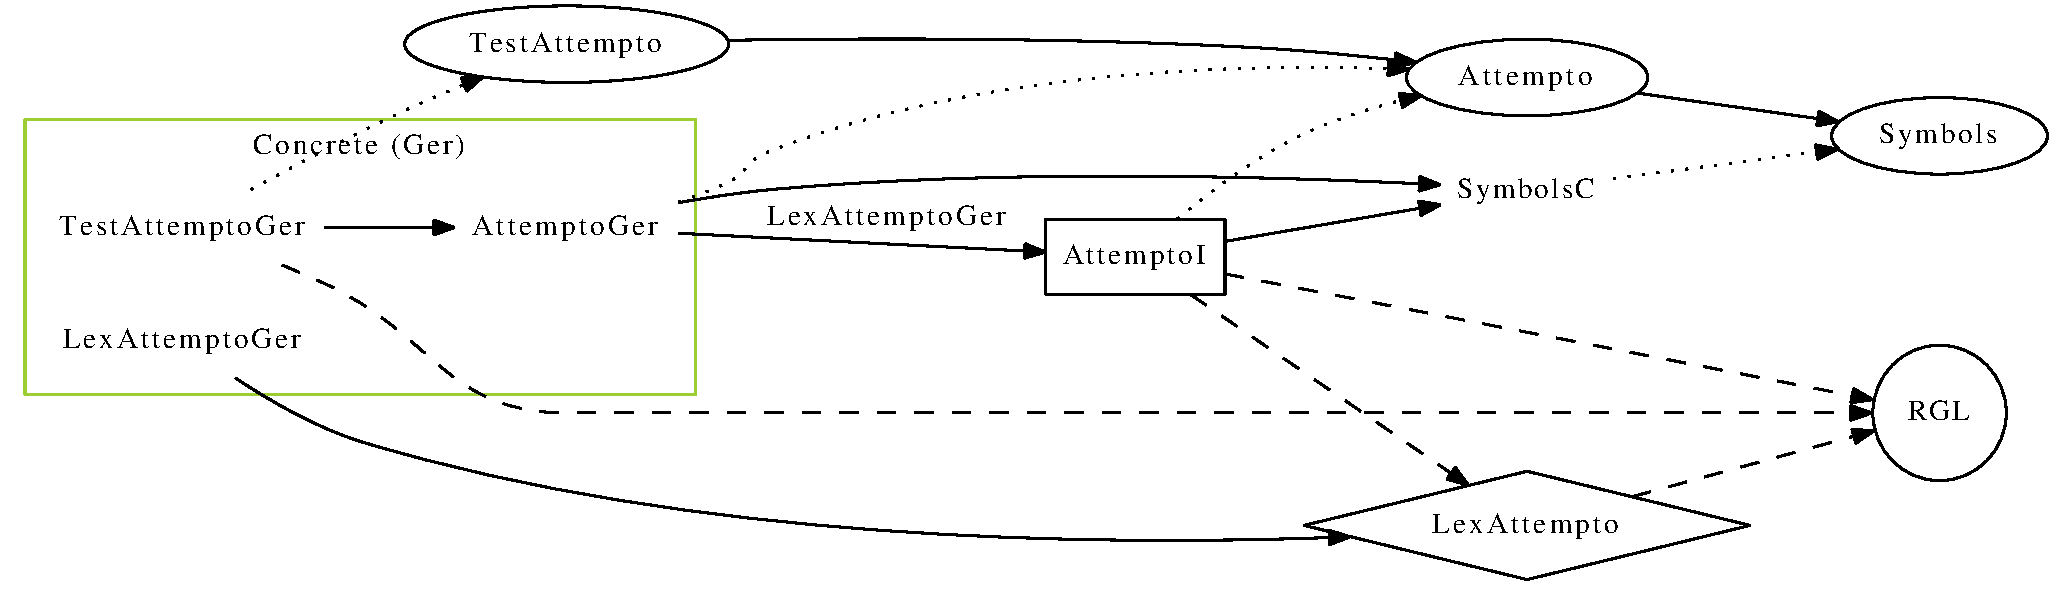
\includegraphics[width=0.99\textwidth]{modules}
\caption[Relations between the ACE grammar modules]
{Relations between the modules, using German (Ger) as an example
of one of the many concrete languages. To add support for a new language,
e.g. Dutch, one must implement three files:
AttemptoDut, which just
instantiates the functor AttemptoI with Dutch-specific resources from the RGL;
TestAttemptoDut, which contains the domain lexicon; and
LexAttemptoDut, which implements the Dutch-specific resources that
do not come from the RGL. The implementation of the lexicon can also
rely on the resources (Dutch morphological paradigms) implemented
in the RGL.}
\label{fig:modules}
\end{figure}

\subsection{Lexicon}

ACE makes a clear separation of lexicon and the rest of the syntax.
The 27 word form types can be added and redefined by the users
\cite{ACE_6.6_Lexicon_Specification}. The AceWiki subset uses a much smaller
but also a slightly different set of lexical categories.

\begin{itemize}
\item proper name (with possible abbreviation and \emph{the}-prefix)
\item common noun (with singular and plural form)
\item noun in an \emph{of}-construct (e.g. `part', `child')
\item transitive verb (with 3rd singular, bare infinitive and past participle
forms)
\item transitive adjective (e.g. `fond of')
\end{itemize}

We map these categories to GF categories as shown in
table \ref{mapping_acewiki_to_gf}.
[TODO: we have to ignore certain things, e.g.  the the-PNs?]

\begin{table}
\begin{center}
\caption{Mapping of AceWiki lexical categories
to GF RGL API categories and GF English
morphological paradigms.\protect\label{mapping_acewiki_to_gf}}
\begin{tabular}{ l l l }
\hline
AceWiki category & GF Cat & GF Eng oper \\
\hline
proper name & PN & \xp{mkPN john} \\
common noun & CN & \xp{mkCN (mkN sg pl)} \\
relational noun & CN & \xp{mkCN (mkN sg \_)} \\
transitive verb & V2 & \xp{mkV2 (mkV go goes \_ gone \_)} \\
transitive adjective & A2 & \xp{mkA2 (mkA fond) (mkPrep of)} \\
\hline
\end{tabular}
\end{center}
\end{table}

%Mapping the ACE lexical categories to GF RGL categories and morphological
%paradigms.
%[TODO: discuss variation]
%
%Table \ref{mapping_clex_to_gf} shows the mapping.
%
%\begin{table}
%\begin{center}
%\caption{Mapping of Clex to GF\protect\label{mapping_clex_to_gf}}
%\begin{tabular}{ r l l }
%\hline
%Clex & Cat & GF oper \\
%\hline
%\xp{noun\_mass} & MCN & \xp{mkCN (mkN ... (mkN ...))} \\
%\hline
%\end{tabular}
%\end{center}
%\end{table}

\section{Multilinguality}

\subsection{GF languages}

We selected the following languages which are supported by the GF RGL.
English, German, Finnish, Urdu, Italian, French, Swedish
(, Hindi, Spanish, Catalan?).

\subsection{ACE vs English}

Does it make sense to treat ACE and English as separate languages in the
grammar, and expose them as different languages to the end user?

\subsection{Main issues}

[TODO: currently copied from \cite{ranta:cnl2009_revised}]
The translation from one language to another using the abstract syntax of the
resource grammar preserves syntactic structure. But it does not always give
the intended result. [TODO: ACE-specific example]
Thus the resource grammar should rather be used as a \emph{library} for
defining the domain grammar. In those cases where direct syntax-based
translation still works (which in practice does cover most cases), a lot of
work can be saved, because the linearization function for a given abstract
function can then be defined once and for all using the language-independent
API of the resource library. Some exceptions to this can then be done for
those languages that do not preserve syntactic structure in translation,
but still using the library. [TODO: example]

\section{Evaluation}

To test the coverage and performance of the GF implementation of the
AceWiki subset we have used
the AceWiki Codeco test set which
is an exhaustive set of sentences with length of up to 10 tokens
(19718 sentences in total).

To test the precision (i.e. possible over-generation) we have used GF's
random generation facility.

To test the correctness of the multilingual translations we have used
the sentences from the
Ontograph
Framework\footnote{\url{http://attempto.ifi.uzh.ch/site/docs/ontograph/}}
\cite{kuhn2009cnlmain}. These sentences cover all the main sentence
patters of the AceWiki subset and they have been used before in user
evaluations of how well the users understand the precise formal meaning
of the sentences.
These 40 sentences cover all the main AceWiki sentence patterns and have
a very clear set-theoretic meaning, e.g.
``Everything that is a traveler or that is an officer sees
at most 1 aquarium.'' means that the union of the sets \emph{traveler} and
\emph{officer} is a subset of the set of all instances that participate in
the 1st argument position in at most one \emph{sees}-relation with an
instance from the set \emph{aquarium}.
The question is if this meaning is understood in the same way via all the
languages.

\subsection{Syntactic coverage}


\subsection{Syntactic precision}

Over-generation is especially undesired in the context of look-ahead editing
\cite{schwitter:eamt-claw2003}, where users would be exposed to
forms which the actual language does not support.

Legal uses of definite NPs cannot be (easily) described in GF, e.g. GF
allows both ``every man likes the man'' and ``every man likes the woman'',
while AceWiki ACE OWL (as implemented in Codeco) allows only the
first one.

[TODO: other interesting cases?]

There are also
places where the AceWiki subset could be extended (rather that its GF
implementation restricted), e.g. AceWiki currently rejects ``every man
likes less than 3 men that own a cat.'' because an NP with a
generalized quantifier (less than 3) cannot be followed by a relative
clause. But this sentence is supported by the ACE-OWL translator
so there is no real reason why it should not be allowed in the
AceWiki subset.

% AceWiki does support: ``... that Mary likes``
Also, support for object relative clauses (``.. that Mary is mad-about'')
is desirable (even though AceWiki does not completely support it).

% AceWiki does not support: who does Mary (not) like?
% (only: Mary likes (does not like) who?)

\subsection{Ambiguity}

[TODO: does the grammar sometimes assign multiple trees to a sentence?]

\subsection{Multilinguality}

[TODO: interesting examples where the straight-forward translation produces
a completely different meaning]

[TODO: the OntoGraph test set does not cover some core ACE equivalences,
e.g. \emph{if-then} equals \emph{every}, double negation equals no negation.
How are these equivalences preserved under the direct syntax-based
translation?]

\subsection{Performance}

[TODO: the GF parser is very fast. Parsing 20k sentences in ?? seconds
and linearizing all of them in 15 languages in ?? additional seconds.]

\section{Availability}

The developed grammar is available under the LGPL license on the GitHub
repository

\begin{quote}
\url{https://github.com/Attempto/ACE-in-GF}
\end{quote}

\section{Future work}

In the
future, one might want to extend the implementation (using
the standard GF extension mechanism) to also cover full ACE.

\bibliography{bib}
\bibliographystyle{alpha}
%\bibliographystyle{plain}

\end{document}
